\documentclass{article}

\usepackage{graphicx}
\usepackage{tikz}
\usepackage{tikzsymbols}
\usetikzlibrary{calc,patterns,shapes.geometric}
\pagestyle{empty}
\usepackage[margin=0pt]{geometry}
\geometry{papersize={14in,12in}}

\def\centerarc[#1](#2)(#3:#4:#5){\draw[#1] ($(#2)+({#5*cos(#3)},{#5*sin(#3)})$) arc (#3:#4:#5);}

\begin{document}
	\begin{figure}
		\centering
		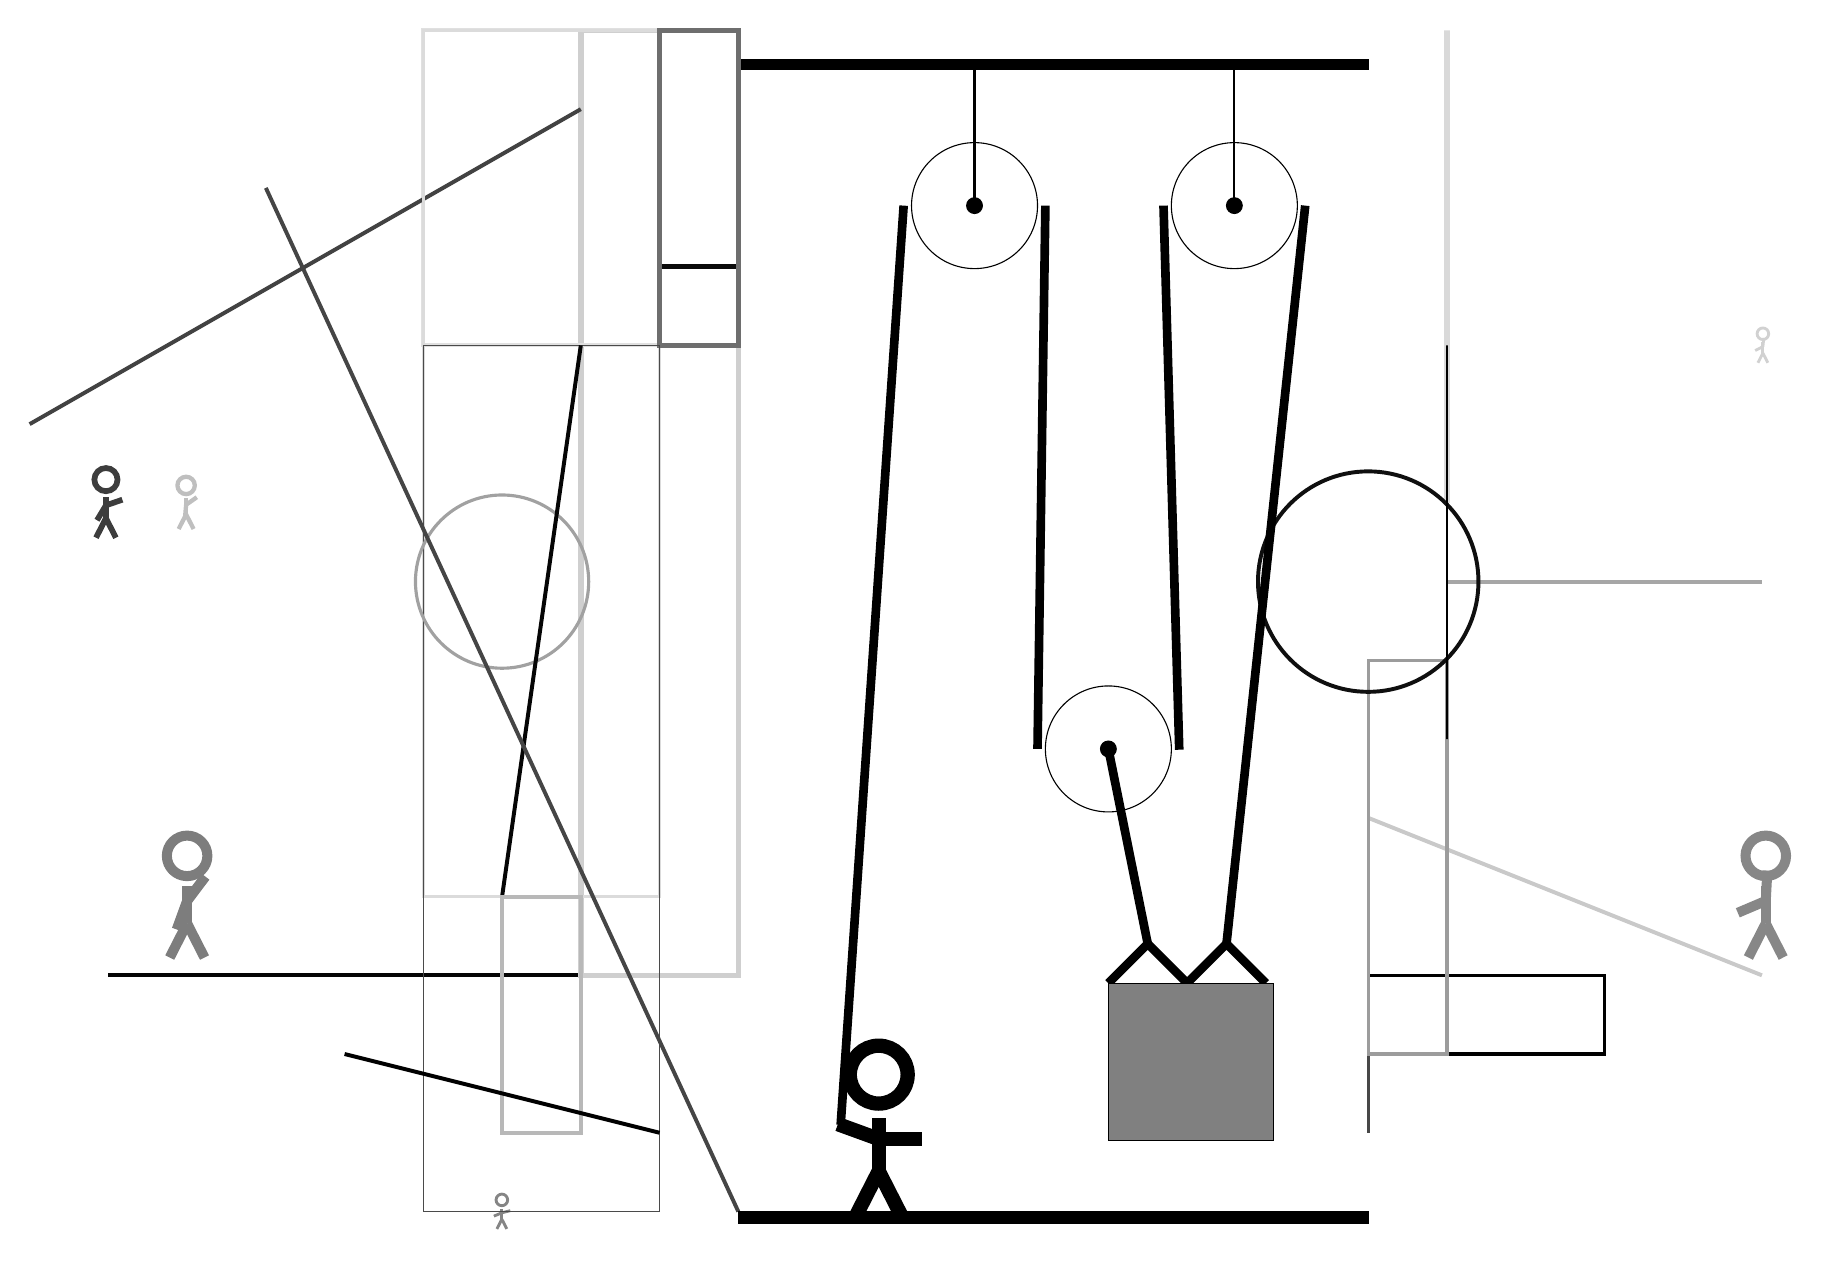
\begin{tikzpicture}
			%%%%% START %%%%%
			
			\draw[fill=black] (-2, 11.5) rectangle (6, 11.625);
			
			\draw (1, 9.775) circle (0.8);
			\draw[fill=black] (1, 9.775) circle (0.1);
			\draw[thick] (1, 9.775) -- (1, 11.5);
			
			\draw[line width=0.5mm, color=black!98](-2, 0) -- (-10, 0);
			
			\node[line width=0.5mm, color=black!18] at (11, 8) {\Strichmaxerl[2][27][84]};
			\draw[line width=0.5mm, color=black!77] (7, 4) rectangle (7, 3);
			\draw[line width=0.4mm, color=black!100] (6, -1) rectangle (9, 0);
			\draw[line width=0.5mm, color=black!21](6, 2) -- (11, 0);
			
			\draw[line width=0.3mm, color=black!64] (-3, 9) rectangle (-3, 5);
			\draw[line width=0.4mm, color=black!72] (6, -2) rectangle (6, 3);
			\node[line width=0.5mm, color=black!51] at (-9, 1) {\Strichmaxerl[7][70][53]};
			\draw[line width=0.7mm, color=black!19] (-4, 0) rectangle (-2, 12);
			\draw[line width=0.5mm, color=black!35](7, 5) -- (11, 5);
			\draw[line width=0.5mm, color=black!12] (-3, 8) rectangle (-6, 12);
			
			\node[line width=0.4mm, color=black!47] at (11, 1) {\Strichmaxerl[7][23][87]};
			\draw[line width=0.4mm, color=black!39] (6, 4) rectangle (7, -1);
			\draw[line width=0.7mm, color=black!15] (7, 6) rectangle (7, 12);
			\draw[line width=0.7mm, color=black!96] (-2, 9) rectangle (-3, 9);
			\node[line width=0.5mm, color=black!25] at (-9, 6) {\Strichmaxerl[3][85][35]};
			
			\draw[line width=0.5mm, color=black!74](-4, 11) -- (-11, 7);
			
			\draw[line width=0.4mm, color=black!14] (-3, 1) rectangle (-6, 12);
			\draw [line width=0.3mm, color=black!22](11, 7) circle (0.0);
			\node[line width=0.6mm, color=black!48] at (-5, -3) {\Strichmaxerl[2][23][14]};
			\draw[line width=0.6mm, color=black!57] (-3, 12) rectangle (-2, 8);
			
			\draw [line width=0.5mm, color=black!94](6, 5) circle (1.4);
			
			\node[line width=0.4mm, color=black!76] at (-10, 6) {\Strichmaxerl[4][59][19]};
			\draw[line width=0.2mm, color=black!71] (-3, 8) rectangle (-6, -3);
			\draw[line width=0.2mm, color=black!100] (7, 3) rectangle (7, 8);
			
			\draw [line width=0.4mm, color=black!37](-5, 5) circle (1.1);
			
			\draw[line width=0.5mm, color=black!98](-5, 1) -- (-4, 8);
			\draw[line width=0.5mm, color=black!73](-2, -3) -- (-8, 10);
			\draw[line width=0.5mm, color=black!28] (-4, -2) rectangle (-5, 1);
			\draw[line width=0.5mm, color=black!100](-3, -2) -- (-7, -1);
			
			\draw (4.3, 9.775) circle (0.8);
			\draw[fill=black] (4.3, 9.775) circle (0.1);
			\draw[thick] (4.3, 9.775) -- (4.3, 11.5);
			
			\draw (2.7, 2.875) circle (0.8);
			\draw[fill=black] (2.7, 2.875) circle (0.1);
			
			\draw[line width=1.1mm]  (2.7, -0.1) -- (3.2, 0.4) -- (3.7, -0.1) -- (4.2, 0.4) -- (4.7, -0.1);
			\draw[fill=black!50] (2.7, -0.1) rectangle (4.8, -2.1);
			
			\draw[line width=1.1mm](-0.7, -1.9) -- (0.1, 9.775);
			\centerarc[line width=1.1mm](1, 9.775)(0:180:0.9);
			\draw[line width=1.1mm](1.9, 9.775) -- (1.8, 2.875);
			\centerarc[line width=1.1mm](2.7, 2.875)(180:370:0.9);
			\draw[line width=1.1mm] (3.6, 2.865) -- (3.4, 9.775);
			\centerarc[line width=1.1mm](4.3, 9.775)(0:180:0.9);
			\draw[line width=1.1mm](4.2, 0.4) -- (5.2, 9.775);
			\draw[line width=1.1mm] (3.2, 0.4) -- (2.7, 2.875);
			
			\node at (-0.2, -2) {\Strichmaxerl[10][-20][0]};
			
			\draw[fill=black] (-2, -3) rectangle (6, -3.15);
			
			%%%%% END %%%%%
		\end{tikzpicture}
	\end{figure}	
\end{document}